\PassOptionsToPackage{hyphens}{url}
\PassOptionsToPackage{usenames,dvipsnames,table}{xcolor}
\PassOptionsToPackage{breaklinks,colorlinks}{hyperref}
\documentclass[usenames, sigconf, 10pt]{acmart}

\usepackage{natbib}
\usepackage{amsmath,amsopn}
\usepackage{graphicx,fancyvrb,multirow}
\usepackage{booktabs}
\usepackage{array}
\usepackage[T1]{fontenc}
\usepackage{fancyhdr}
\let\labelindent\relax
\usepackage[labelfont=bf,font=small,skip=5pt]{caption}
\pagestyle{fancy}
\fancyhf{}

\usepackage{fp}
\usepackage{balance}
\usepackage[ruled, vlined, inoutnumbered, linesnumbered]{algorithm2e}
\usepackage[titletoc]{appendix}

\usepackage{color}
\definecolor{lightgray}{rgb}{0.92, 0.92, 0.92}
\definecolor{darkgray}{rgb}{0.4, 0.4, 0.4}
\definecolor{editorOcher}{rgb}{1, 0.5, 0}
\definecolor{darkgreen}{rgb}{0,0.45,0}
\definecolor{codeblue}{rgb}{0,0,0.55}
\definecolor{darkred}{rgb}{0.8,0.1,0.15}
\definecolor{codegray}{rgb}{0.5,0.5,0.5}

\usepackage{listings}
\lstset{
  language=PHP,
  backgroundcolor=\color{white},
  basicstyle=\fontsize{7}{9}\ttfamily,
  breakatwhitespace=false,
  breaklines=true,
  captionpos=b,
  commentstyle=\color{codegray},
  deletekeywords={...},
  escapeinside={\%*}{*)},
  extendedchars=true,
  frame=bt,
  keepspaces=true,
  keywordstyle=\color{darkgreen}\bfseries,
  ndkeywordstyle=\color{editorOcher}\ttfamily,
  morekeywords={*,...,string,=>,function,<?,php, NULL},
  numbers=left,
  numbersep=7pt,
  numberstyle=\footnotesize\color{darkgray}\ttfamily,
  rulecolor=\color{black},         
  showspaces=false,
  showstringspaces=false,
  showtabs=false,
  stepnumber=1,
  stringstyle=\color{darkred}\ttfamily,
  tabsize=2,
  title=\lstname,
  firstnumber=1,
  identifierstyle=\color{codeblue},
  xleftmargin={2em},
  framexleftmargin={2em},
}


\newcommand{\sys}{\mbox{\textsc{XSym}}\xspace}

% ref. http://en.wikibooks.org/wiki/LaTeX/Colors
\newcommand{\WM}[1]{\textcolor{Violet}{[WM: #1]}}
\newcommand{\PENGHUI}[1]{\textcolor{blue}{[PENGHUI: #1]}}
\newcommand{\KL}[1]{\textcolor{Magenta}{[KL: #1]}}
\newcommand{\XX}[0]{\textcolor{red}{XXX}\xspace}
\newcommand{\XXX}[1]{\textcolor{red}{XXX: #1}}
\newcommand{\TODO}[1]{\textcolor{Melon}{TODO: #1}}

\newcommand{\totalfuncnum}{320\xspace}
\newcommand{\navex}{Navex\xspace}
\newcommand{\navexnum}{35\xspace}
\newcommand{\funcnum}{287\xspace}

\newcommand{\num}[1]{#1}
\newcommand{\cc}[1]{\mbox{\smaller[0.5]\texttt{#1}}}
\def\Snospace~{\S{}}
\renewcommand*\sectionautorefname{\Snospace}
\def\sectionautorefname{\Snospace}
\def\subsectionautorefname{\Snospace}
\def\subsubsectionautorefname{\Snospace}

\newcommand{\eg}{{\em e.g., }}
\newcommand{\etal}{{\em et al.}}
\newcommand{\etc}{{\em etc.}}
\newcommand{\ie}{{\em i.e., }}

\newcommand{\PP}[1]{
\vspace{2px}
\noindent{\bf \IfEndWith{#1}{.}{#1}{#1.}}
}

\newcommand{\PN}[1]{
\vspace{2px}
\noindent{\bf #1}
}

\settopmatter{printacmref=false, printccs=false, printfolios=false}
\setcopyright{none}
%\setcopyright{iw3c2w3}
\copyrightyear{2021}
\acmYear{2021}
\acmConference[CSCI '5570]{Large Scale Data Processing Systems}{Spring 2021}{CUHK}
\acmBooktitle{Large Scale Data Processing Systems}
\acmPrice{}
\acmDOI{}
\acmISBN{}


\begin{document}
\title[]{Understanding and Detecting Bugs in Network Operating Systems}

\author{Penghui Li 1155137827}
\email{phli@cse.cuhk.edu.hk}
\settopmatter{printacmref=false, printccs=false, printfolios=false}
\setcopyright{none}
%\setcopyright{iw3c2w3}
\copyrightyear{2021}
\acmYear{2021}
\acmConference[CSCI '5570]{Large Scale Data Processing Systems}{Spring 2021}{CUHK}
\acmBooktitle{Large Scale Data Processing Systems}
\acmPrice{}
\acmDOI{}
\acmISBN{}



\begin{abstract}
Network systems connect the Internet world.
Bugs in network systems can lead to denial-of-service, performance issues, \etc{}
Understanding network system bugs can benefit both the system developers and security analysts.

However, to the best of our knowledge, the bugs in network systems have not been well understood. 
    The potential security impact has not been well investigated as well.
    In this project, we aim to understand the bugs in network systems. 
    We hope to learn lessons to further guide future bug detection in network systems.
\end{abstract}


\maketitle
\sloppy


%\section{Introduction}
\label{s:intro}
Network Operating Systems (NOSs) connect multiple computers and devices and manage network resources in the settings of Software Defined Networking (SDN).
%
NOSs manage multiple requests concurrently and provide the security in multiuser environments. 
%
To date, there are many NOSs being proposed and matained by network service vendors.
%
For example, Cisco Internetwork Operating System is a family of network operating systems used on many Cisco Systems routers and current Cisco network switches \cite{edgeworth2014ip};
DD-WRT \cite{dd-wrt} is a Linux based open-sourced NOS suitable for various WLAN routers and embedded systems.
%
%

Due to their popularity and critical uses, the bugs in these network operating systems can lead to severe security consequences.
%
In particular, network operating systems could have performance bugs, which cause excessive resource consumption and could negatively affect user experiences.
%
They can be further leveraged by attackers for launching application-layer denial-of-service (DoS) attacks \cite{crosby2003algodos}.
%
By specially crafting inputs to trigger a performance bug in the network operating systems,
%
the attacker can exhaust the server's resources (\eg{,} memory and CPU) and make the services unavailable to normal users. 

%
To the best of our knowledge, there currently has little knowledge about the prevalence of performance bugs in the wild.
%performance bugs.
%
Prior studies on compilers generally focus on memory corruptions,
%
whereas performance bugs, especially in close-sourced network operating systems, are not well investigated and understood yet.
%
Some works studied performance issues in the regular expression engines \cite{shen2018rescue,wustholz2017static}, desktop software \cite{perfbugstudy}, and Android applications \cite{liu2014characterizing}.
%
Network operating systems, however, have not been covered.
%
To this end, we conduct a comprehensive study of the performance bugs in network operating systems to answer the following research questions:
%
\begin{itemize}[itemsep=0.5ex, parsep=0ex, leftmargin=3mm]
    \item What are the main categories of the bugs?
    \item What are the main factors that cause bugs?
    \item How widespread are the bugs in network operating systems?
    \item How severe are the bugs in network operating systems?
\end{itemize}

We empirically analyze \XX known performance bugs in mainstream network operating systems and thoroughly summarize their characteristics.
%
We observe that there has been a continuous growth in the number of reported performance bugs in the past 3 years.
%
We further identify that the ways that network operating systems handle the language's context-sensitive features are the dominant root cause of the performance bugs.
%
We reveal that the developers of network operating systems usually mitigate such exploitation by enforcing a hard limit for the maximum number of backtracking for certain tasks, which, however, limits the intended functionality of the network operating systems.


In this work, we also explore detecting performance bugs in network operating systems.
%
To the best of our knowledge, there is not any tailored tools specially designed for detecting performance bugs in network operating systems.
%
Fuzzing \cite{slowfuzz, hotfuzz, perffuzz} eliminates the limitations of static analysis techniques 
(\eg{,} high false positives) 
\cite{perfbugstudy, nistor2013toddler,nistor2015caramel}.
%
It has become the go-to approach with thousands of vulnerabilities in real-world software.
%
Without a doubt, performance bugs in network operating systems can be fuzzed as well.
%
%However, existing fuzzers \cite{slowfuzz, perffuzz} for performance bugs are not aware of special \emph{contex} of network operating systems and cannot effectively generate inputs to thoroughly exercise them.
%
%Therefore, besides the bit/byte level mutation \cite{afl}, we summarize the rules of the inputs. 
%
%We develop a syntax-tree based mutation strategy \cite{superion} to preserve and extend useful rules during the input mutation.
%
%This helps to generate inputs more effectively.
%
%

We mainly focus on CPU exhaustion performance bugs.
%
To detect them, we monitor the program execution under the generated inputs.
%
We employ a statistical model using Chebyshev inequality to label abnormal cases as performance bugs.
%
This can potentially cause duplicate bug reports as multiple bug reports with only slight difference in the inputs actually trigger the same bug.
%
It is time-consuming and impractical to leverage human efforts to manually de-duplicate them.
%
Existing bug de-duplicating methods using coverage profile and call stacks are inaccurate and not applicable to performance bugs.
%
For example, it is hard to obtain an accurate and deterministic call stack that reveals the situation when a performance bug is triggered.
%
Therefore, we propose a execution trace similarity comparison algorithm to de-duplicate the reports.
%
Specifically, we represent the execution trace of each report into a vector;
%
we compute the cosine similarity between vector pairs and classify vectors (bug reports) with high similarity as the same bug.
%

We integrate abovementioned techniques into \sys.
%
We demonstrated \sys outperformed the state-of-the-art works \cite{slowfuzz, perffuzz} \emph{better} performance slowdown, and \emph{higher} code coverage.
\sys is highly effective in generating test cases to trigger new code in the testing network operating systems.
%
Though we have not identified any new bugs yet after 6-hour testing, we plan to further keep \sys running for more time.
%
Hopenfully, our techniques can help find new bugs in the future.

In summary, we make the following contributions in this work.
\begin{itemize}
    \item
        We conduct a systematic study on performance bugs in network operating systems.
        %
        We present an empirical understanding of the performance bugs and the patches.
        %
    \item We develop a new system, \sys, to effectively generate useful inputs to detect performance bugs in network operating systems.
        %
    \item We demonstrate \sys can significantly outperform the state-of-the-art works.
\end{itemize}

\section{Network System Bugs}

Network systems are the hardware and software components from which these networks are built \cite{serpanos2011architecture}.
They are commonly applied to perform data analytics, e-commerce, storage back, \etc{} \cite{gill2011understanding}.
The network architectures have been involved rapidly along with the advance of new network applications, \eg{} video applications and video streaming.

Bugs commonly exist in network systems.
For example, more than 200 bugs were found in the Linux IP stack \cite{bugzilla}.
Such bugs can cause severe security and reliability problems like crashes, denial-of-service, and failures \cite{gill2011understanding}.

Understanding the root causes of the bugs in network systems is important.
In particular,
first, the empirical knowledge can benefit system developers to avoid making similar mistakes.
Second, security analysts are thus possible to design new approaches to identifying bugs.
The network systems thus can be more secure and reliable.
The user experience can be significantly improved as well \cite{user-exp}.

\section{Related Work and Research Problems}
There are substantial works on characterizing different types of bugs in many systems  (\eg{} regular-expression denial-of-service bugs in web applications \cite{perfbugstudy, nistor2013toddler,nistor2015caramel}, performance bugs in C/C++ compilers \cite{sun2016toward, yang2011finding}).
Such studies greatly advance the improvement of security analysis and bug detection techniques.
For example, Yang \etal{}, guided by their empirical study, developed a rule-based static system to effectively and scalably detect new bugs in C/C++ compilers.

Toward understanding bugs in network systems, Yin \etal{} studied the bugs in open-sourced router software \cite{yin2010towards}.
They concluded the many bugs could lead to reliability issues and were hard to patch.
Gill \etc{} investigated bugs in data center networks and demonstrated that the load balancers were highly buggy \cite{gill2011understanding}.
However, to the best of our knowledge, these works either fall short of characterizing the root causes of the bugs or have not included newer network software.
Furthermore, how such knowledge can benefit the security analysis has not been demonstrated yet.

In this project, we plan to conduct a comprehensive study on existing bugs in several network systems.
Specifically, we aim to answer the following research questions:
\begin{itemize}
\item What are the main categories of the bugs?
\item What are the main factors that cause bugs?
\item How widespread are the bugs in network systems?
\item How severe are the bugs in network systems?
\end{itemize}

Second, we hope to summarize the general patterns of the bugs in network systems and the common practices in patching network system bugs.

Note that, 
there is no guarantee that we are able to design a better tool to detect network system bugs or not as this largely depends on what we find in the empirical study, which is unknown for now.
We do not promise we will be able to identify new bugs within this project.
Nevertheless, the empirical knowledge on network system bugs can definitely benefit the community to develop more secure and reliable network systems.


\section{Logistics}
Regarding the time of \emph{6 weeks} for this project, we plan to use \emph{3 weeks} on understanding existing bugs in network systems; 
we then spend \emph{2 weeks} on summarizing the bugs and implement necessary tools (if available) for more practical bug detection;
last, we use \emph{1 week} to present our findings in the final reports.
The time schedule is tentative and might change accordingly.

As required, we currently host the project content on a GitHub page\footnote{https://peng-hui.github.io/csci5570-project.html}.
We also create on a GitHub repository\footnote{https://github.com/peng-hui/csci5570-project} and will maintain the necessary project artifact (\eg{} source code (if any), dataset) there.

%\section{Background}
\label{s:background}

\subsection{Performance Bugs}
\label{s:background-bug}
%\TODO{Have not had time to rephrase the decriptions from 'parser'->'compiler'}
Performance bugs in a program could degrade its performance and waste computational resources.
%
Usually, people define performance bugs as software defects where relatively simple \emph{source-code} changes can significantly optimize the execution of the software while preserving the functionality \cite{perfbugstudy, killian2010finding, s2e}.
%
There can be several different performance issues regarding different categories of resources.
%
For example, some performance bugs could cause excessive CPU resource utilization, resulting in unexpectedly longer execution time; 
%
some other bugs could lead to huge memory consumption because of uncontrolled memory allocation and memory leak \cite{wen2020memlock}.
%

%they 
Performance bugs lead to reduced throughput, increased latency, and wasted resources in software.
%
They particularly impact the end-user experiences.
%
What is worse, when a buggy application is deployed on the web servers, the bugs can be exploited by attackers for denial-of-service attacks, which can impair the availability of the services \cite{rampart}.
%
In the past, performance bugs have caused several publicized failures, causing many software projects to be abandoned \cite{perfbugstudy, lessons}.

\subsection{Network Operating Systems}
\label{s:background-nos}
Network operating system is a computer operating system that facilitates to connect and communicate various autonomous computers over a network. 
%
An autonomous computer is an independent computer that has its own local memory, hardware, \etc{}
%
It is self capable to perform operations and processing for a single user. 
%
Network operating systems can be embedded in a router or hardware firewall that operates the functions in the network layer \cite{al2001dialoguer}.
%
Typical real-world network operating systems include Cisco IOS \cite{cisco-ios}, DD_WRT \cite{dd-wrt}, Cumulus Linux \cite{cumulus-linux}, \etc{}



%\section{Understanding Performance Bugs} 
\label{s:study}
%To the best of our knowledge, there is currently little knowledge about 
%
In this section, we present an empirical study on several known performance bugs in mainstream network operating systems 
to help understand their characteristics. % of the performance bugs. % in Markdown compilers.
%

\subsection{Data Collection}
\label{s:study-bug}

\iffalse
\begin{table}[t]
\centering
    \caption{The existing performance bugs included in our study.
    %Lang. means the underlying programming language for implementing the Markdown compiler.
    }
\label{table:study-dataset}
\small
%\resizebox{0.47\textwidth}{!}{
\begin{tabular}{lcc}
   \toprule
      Software  & \# Bugs & Time Periods \\
    \midrule
    Cicso IOS \cite{cicso-ios} & 58 & 10/26/2001 - 01/13/2021 \\
     & & 01/14/2017 - 12/20/2020 \\
    MD4C & 6 & 03/10/2019 - 09/10/2019\\
    commonmark.js & 9 & 09/28/2017 - 08/13/2019 \\
    markdown-it & 8 & 08/14/2019 - 11/20/2020\\
%    \midrule
%    Total &  & (49) 52 & 10/26/2014 - 12/20/2020\\
   \bottomrule
\end{tabular}
%}
\end{table}
\fi

%As shown in \autoref{table:study-dataset}, 
%
We investigate performance bugs in the Cicso IOS \cite{cicso-ios}, 
%
which is one of the most popular network operating systems.
%
Ideally, if more network operating systems are included in the study we can present a more comprehensive characteriazation.
%
However, due the the limited time and human labours allowed for this work,
%
we have to somehow restrict the study scope.
%
Nevertheless, this work, as an early stage studying performance bugs in network operating systems, shall provide some general inspirations for future network system security analysis.

We manually collected 58 distinct performance bugs from the database of Common Vulenrabilities and Exposures (CVE) \cite{cve}.
%
The detailed information about the vulnerabilities included in our study is presented in \autoref{cve-details}.
%
Some bug reports might be duplicates.
%
We remove a duplicate bug from our dataset if it has a similar cause as another one,
%
though it can have a different exploit vector.
%
In summary, we obtained 49 distinct performance bugs by removing \XXX duplicates from the ones reported from November 2001 to January 2021.
%
We found all these performance bugs were abusing the CPU resources or memory resources.
%
%This suggests CPU resource exhaustion performance bugs are the dominant type of performance bugs.

We next characterize the performance bugs and present our findings.

\subsection{Bug Disclosure Over Time}
\label{s:study-time}

\begin{figure}[t]
    \centering
    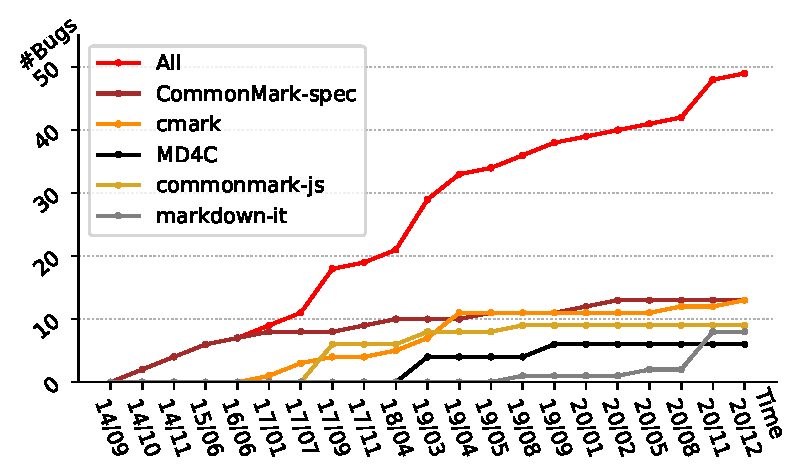
\includegraphics[width=0.45\textwidth, trim =5 0 0 0,clip]{fig/disclosure-time.pdf}
    \caption{The number of performance bug reports over time.
    }
    \label{fig:disclosure-time}
\end{figure}

To understand the trend of performance bugs, we analyze the disclosure time of them.  
We depict the number of performance bugs along the time they were disclosed in \autoref{fig:disclosure-time}.
%
We observe that few bugs were reported before early 2004, and the number of reported bugs had been gradually growing from early 2018 till late 2020.
%
In particular, 28 (57.14\%) out of the 49 performance bugs were disclosed from April 2018 till December 2020 (22 months);
%
21 (42.86\%) bugs were reported from August 2014 to December 2017 (41 months).
%
It reveals that such bugs had been gradually drawing the attention from the compiler developers and security analysts.
%

\subsection{Root Causes}
\label{s:study-root-causes}
%
Identifying the common root causes of real-world performance bugs can benefit potential future research and software developments.
%
We manually analyzed the performance bugs and successfully figured out the root causes for \XX bugs.
%
We classify the root causes into three categories.
%
A bug is assigned to multiple categories if it has multiple major causes.


\PN{R1:} \emph{Super-linear algorithms.}
Some normal algorithms implemented in Markdown compilers have super-linear worst-case complexity \cite{slowfuzz, perffuzz}.
%
Attackers can craft inputs to trigger the worst-case behaviors and lead to performance issues.
%
%For instance, some compilers use regular expressions to match inputs, which are vulnerable to ReDoS attacks \cite{redos} that trigger excessive numbers of backtracking in the matching process.
%
The majority (25 out of 39) of bugs were related to such worst-case behaviors.
%\WM{Check this number again after moving ReDoS to R2.}
%
%Specifically, the abnormal backtracking logic in Markdown compilers can be further divided into two groups:
%
%
%Known performance bugs in this category exploit either the design of Markdown compilers or the vulnerable regular expression and can lead to polynomial or exponential complexity compilation time.
%
%What is worse, the intended normal functionality of the Markdown compilers can be abused by crafted inputs for triggering worst-case behaviors, \eg{,} excessive number of backtracking.
%
%This includes triggering cataphoric backtracking in regular expression matches and the similar logic design inside the Markdown compilers can be abused with specially crafted inputs.
%
%
%If the input size is not limited, the Markdown compilers can easily hang for up to several hours.
%
%
%27 out of 39 performance bugs belong to this category.
%Specially crafted inputs abuse the backtracking behaviors and lead.
%
%We investigate the specially crafted inputs that lead to such worst-case behaviors. %and present two bugs in this category.
%We discuss two primary kinds of algorithms that exhibit the super-linear worst-case complexity we find. % in the Markdown compilers.
%
%They can be roughly divided into two groups:
%
%(1) long open tokens without close tokens,
%
%and (2) long early open tokens and late close tokens.
%

Some Markdown syntaxes (\eg{,} links, emphasis and strong emphasis, HTML blocks) are related to the language's context-sensitive features.
%
%We notice that the performance bugs are quite related to the logic (syntax) of the Markdown language,
%
%in particular, its context-sensitive features.
%
As discussed in \autoref{s:background-compiler},
supporting context-sensitive features in Markdown requires the compilers to backtrack, which could take more than linear time.
%
The backtracking strategies can easily be abused with crafted inputs hence lead to performance issues.
%
%\WM{Check the following. The total number 25+14 are larger than the above 27.}
For instance, links were the primary vulnerable syntax in Markdown compilers,
%
where 11 of the known performance bugs could be exploited with special inputs with links.
%
%Usually, they can happen together with other syntax components.
%
%
%Emphasis and strong emphasis is the second vulnerable Markdown syntax.
%HTML blocks are also the most vulnerable Markdown syntax component in Markdown compilers.
%
Similarly, 8 of the bugs were caused by the buggy emphasis and strong emphasis handlers.
%
Our study reveals that the implementation of the context-sensitive features in the Markdown compilers are prone to containing performance bugs.
%For example, the backtracking from wrong options can be abused and result in performance issues.



One typical input pattern that exploits the context-sensitive syntax handler to trigger performance bugs is \emph{many open tokens}.
%
This pattern can lead the compilers to repeatedly search a close token towards the end of the input string for each such open token, and also force the compilers to backtrack to correct wrong options the compilers have selected.
%
%Regarding the number of repetitions, $n$, the time complexity can be $O(n^2)$ or higher.
%Some logic design of Markdown compilers produces similar backtracking behaviors when a temporal mismatch is detected.
%
For example, deeply nested CDATA block open delimiters can result in an excessive compilation time.
%
%When Markdown compilers detect the first CDATA block open delimiter (\ie{,} \blstinline{<![CDATA[}), they have to search to the end until a matched CDATA block close delimiter (\ie{,} \blstinline{]]>}) is found.
%
%When the match cannot be found, the Markdown compilers perform backtracking to the current CDATA open delimiter.
%
When fed with $n$-nested CDATA block open delimiters (\eg{,} \blstinline{'<![!CDATA[<![CDATA[<![CDATA[...'}) that are not closed with the corresponding close delimiters (\ie{,} \blstinline{']]>'}) or are closed in the end of the input string,
%
%can backtrack repeatedly on every open delimiter and in total for $n$ times.
the compilers need to compare with all tokens in the input string to determine if an open delimiter can be closed or not.
%
Once the compilers find an open delimiter cannot be closed, they switch to other possible options for that delimiter next, for instance, the open delimiter \blstinline{'<!'} in \blstinline{'<!A>'}, which cannot be closed either.
%
%Each time, the compilers have to search till the end of the input string.
%
Thus the time for handling such input strings is at least in polynomial time complexity.
%
By providing a long input with many such open tokens, it is simple to cost the compiler several-second or even more execution time.
%Depending on how such backtracking strategies are designed, such inputs can cause polynomial or higher complexity performance issues, easily resulting in seconds of execution time.


\PN{R2:} \emph{Inefficient code.}
%
Some inefficient code in the Markdown compilers could also lead to performance issues.
%
For instance, some functions do not coordinate well for certain functionalities.
%
We find that 9 performance bugs were caused by such inefficient code.
%
Unlike the algorithms in R1, such performance issues could be addressed by optimizing the inefficient code.
%
However, each problem needs to be separately analyzed and fixed, which could be time-consuming.
%
We next discuss an example of such inefficient code.
%

Minor performance issues in individual problematic functions could accumulate when the given inputs can repeatedly trigger the execution of such functions.
%
For example, in one bug, cmark calls \blstinline{S_find_first_nonspace()} to find the first non-space character from the current offset in a line. %, which has a minor performance issue by
%
%The function went back from the current offset backwardly to find the first non-space character,
The function in a second call would still search from the initial position,
even if in a previous call it has already recognized the location of the first non-space character.
%
This means some function calls to \blstinline{S_find_first_nonspace()} sometimes were unnecessary.
%
Crafted inputs with lots of complicated and nested indents could result in repeated invocations of this function and cause performance bugs.
%
The problem, however, can be solved by using better strategies like cashing the positions of the previously found non-space characters.
%

\iffalse
Second, some Markdown compilers match input strings using regular expressions (regex).
%
Some vulnerable regex could lead to performance bugs if the regex engine needs to backtrack (in exponential time) when matching some specific inputs.
%
A failed matching attempt can lead the engine to backtrack with multiple choices.
%
Thus the total number of possible backtracking paths is exponential if the match cannot be found eventually for every input symbol.
%
This is also known as regular expression denial-of-service (ReDoS) \cite{freezing, shen2018rescue, redosimpact, wustholz2017static}.
%
For instance, one bug in commonmark.js was caused by using a regex containing a vulnerable subexpression \blstinline{(.|\\\\)*]}\footnote{The vulnerable subexpression is simplified for demonstration.}
to match link labels (\eg{}, the \blstinline{[demo]} in \blstinline{'[demo](url 'title')'}).
%
Its syntax is to match any non empty character \blstinline{.} or a single blackslash \blstinline{\\\\} for any number of times \blstinline{*}, followed by a closing bracket \blstinline{]}.
%
%
Suppose the compiler uses this regex to match an input string \blstinline{'\\\\\\\\...'} that contains $n$ backslash characters.
%
The matching would eventually fail because the input string does not contain any closing bracket.
%
But before the failure, the regex engine would check all possible matches for the previous part \blstinline{(.|\\\\)*}.
%
%
Each backslash character in the input string can match either \blstinline{.} or \blstinline{\\\\}, so $n$ characters would cause the engine to backtrack with $2^n$ possible paths.
%
Nevertheless, such performance bugs could be addressed by fixing the vulnerable regex.
\fi
%

\PN{R3:} \emph{Implementation-specific issues.}
Other causes of the bugs are specific to the compiler implementations or designs.
%
Some compilers overlooked part of the CommonMark specification, for example, Unicode support.
%
This can lead to infinite loops when unexpected inputs are provided to the compilers.
%
Some other bugs in this category were caused by wrong data structures.
%
5 performance bugs fall into this category.

\begin{comment}
\subsection{Markdown Syntax and Performance Bugs}
\label{s:study-markdown}

\begin{table}[t]
\caption{Top 4 types of vulnerable Markdown syntax}
\label{tab:bug-syntax}
\centering
\small
\resizebox{0.47\textwidth}{!}{
\begin{tabular}{lcll}
    \toprule
    Markdown syntax & Bugs & Examples  & Root causes\\
    \midrule
    Links & 25 & \blstinline{'[ (]( [ (]( ...'} & \textbf{R1} \textbf{R2} \textbf{R3} \\
    (Strong) Emphasis &14 & \blstinline{'a\_ a\_ ...'} & \textbf{R1} \textbf{R3}\\
    HTML blocks & 9 & \blstinline{'<!\[CDATA\[ <![CDATA[...'} & \textbf{R1} \\
    Fenced code blocks & 5 & \blstinline{'```\\ncode\\n...'} & \textbf{R1}\\
   \bottomrule
\end{tabular}
}
\end{table}

%

We investigate the relationship between the Markdown syntax and the compiler performance bugs.
%
We present the top 4 types of vulnerable Markdown syntaxes of the known performance bugs in \autoref{tab:bug-syntax}.
%
A bug is classified into one or multiple syntax groups if it is caused by the inefficient or incorrect implementations of the syntax(es).
%
%A bug can be classified into several syntax groups if it breaks several syntax handlers.
%
We also list an example for each syntax group in the third column of \autoref{tab:bug-syntax}.
%


We also show the main root causes in each syntax component in the last column of \autoref{tab:bug-syntax}.
%
We include the root cause for a syntax group if at least one bug in the group has that root cause.
%
The results show that unlimited backtracking behaviors were quite common---all the top 4 buggy Markdown syntax components contained bugs with such a root cause.
\WM{<- Check this backtracking.}

\end{comment}

\iffalse
\subsection{Patches of Performance Bugs}
\label{s:study-patch}
We investigate the patches of performance bugs in Markdown compilers to understand how they were addressed.
%
We manage to identify the bug fix patterns for 28 performance bugs.
%
We present our findings below.
%

\PN{P1:} \emph{Enforcing limits.}
%
The most common patch pattern is to add limits for certain conditions such as the maximum depth of the nested structure,
%
although the CommonMark specification does not explicitly specify any such limits.
%
%
When such limits are reached, the compilers directly regard the rest unanalyzed inputs as plain text.
%
%Most uses of Markdown compilers normally do not exceed such limits,
%
%\eg{}, the depth of nested parenthesis seldom reaches thousands of layers.
%
Enforcing limits can prevent excessive CPU usages caused by the worst-case exploitation of too large test cases.
%By adding a limit,
%
However, 
the intended functionality might be violated.
%
It is also difficult to set a correct limit to prevent all attacks while not breaking some unusual yet legitimate inputs.
%the Markdown compilers will abort the tasks and process other tasks if a certain limit is reached.
%
%Such a strategy is simple yet useful.
%
Such a strategy has been applied to patch 13 out of the 28 bugs we investigate.

\PN{P2:} \emph{Logic changes.}
Logic changes sometimes are necessary as the bugs are caused by the incorrect coordination among multiple program components and functions.
%
Some inefficient code snippets need to be further optimized to eliminate the underlying performance issues.
%
For some other performance bugs caused by incorrect regular expressions,
compiler developers mainly review and rewrite the regular expressions.
\fi

%\input{performance}
%\section{Limitations}
This work has several limitations that need to be further addressed.
%
First, we failed to instrument some network operating systems for the evaluation and alternatively evaluated in other systems.
%
This problem, was out of the foreseeable scope of the authors when proposing the idea.
%
The authors also were not able to fix it given limited time.
%
Though our technique is general, there might be some unknown challenges that we cannot foresee now.
%
We have to tackle this limitation to make \sys applicable for our initial purposes.
%
Nevertheless, our evaluation somehow demonstrated the efficacy of \sys.
%
Similarly, we are in certain confidence that \sys can also perform excellently once the above challenge is solved. 
%
Second, also due to the lack of human efforts, the empirical study is deep enough.
%
There are many other interesting aspects that can be studied further.
%
For example, how are the performance bugs patched?
%
We will further investigate these directions in the future.


%\section{Conclusion}
\label{s:conclusion}
Performance bugs in network operating systems are previously understudied.
%
This paper conducted a systematic study to understand the characteristics of the performance bugs.
We designed \sys with several new techniques to detect performance bugs in the wild.
%
Our evaluation demonstrates report de-duplication is necessary and our solution is effective.
%
We hope our research, as an initial step, can shed some light on future security analysis and software developments.


\balance
%\interlinepenalty=10000
\bibliographystyle{sty/ACM-Reference-Format}
%\footnotesize
%\setlength{\bibsep}{3pt}
\bibliography{p,conf}
\end{document}
